\documentclass[small,xcolor=svgnames]{beamer}
%\documentclass[handout]{beamer}
%compress

\usepackage[latin1]{inputenc}
\usepackage[english]{babel}

\usepackage{colortbl}
\usepackage{amsmath}
\usepackage{amssymb}
\usepackage{latexsym}
\usepackage{ifpdf}
\usepackage[all]{xy}
\usepackage{graphics}
\usepackage{color,xcolor,ucs}

\setbeamertemplate{footline}[frame number]

%%%%%%%%%%%%%%%%%%%%%%%%%%%%%%%%%%%%


\font \Bbb=msbm10 scaled \magstep1
\def\a{\alpha}
\def\A{{\mathcal{A}}}
\def\b{\beta}
\def\bs{\bigskip}
\def\Box{$ \hspace{13cm}  \fbox{}$\\}
\def\cu{\mbox{{\rm\bf curl}\,}}
\def\Cu{\mbox{\rm Curl\,}}
\def\Curl{\mbox{\rm Curl\,}}
\def\d{{\rm d}}
\def\D{D}
\def\di{\mbox{\rm div\,}}
\def\Di{\mbox{\bf Div\,}}
\def\div{\mbox{\rm (div)}}
\def\divd{\mbox{\rm (div)}_2}
\def\divw{\mbox{\rm (div)}_{p,\omega}}
\def\divdw{\mbox{\rm (div)}_{2,\omega}}
\def\dom{d_{\Omega}}
\def\e{\ve}
\def\f{{\mathrm{F}}}
\def\ff{{\bf f}}
\def\g{\gamma}
\def\G{{\bf G}}
\def\H{{\mathcal{H}}^{N-1}}
\def\hb{\hat{\beta}}
\def\hg{\hat{g}}
\def\ho{\hat{\Omega}}
\def\hoj{\ho^{n^\prime,s}}
\def\hw{\hat{w}}
\def\hx{\hat{x}}
\def\hy{\hat{y}}
\def\hz{\hat{z}}
\def\hzp{\hz^\prime}
\def\I{{\mathcal{I}}}
\def\J{{\mathcal{J}}}
\def\jep{{\mathcal J}_\ep}
\def\K{{\mathcal{K}}}
\def\l{\ell}
\def\lp{L^p(\partial\Omega)}
\def\L{{\bf L}}
\def\Li{L^{\infty}}
\def\Lp{L^p(\o)}
\def\Lq{L^q(\o)}
\def\Linf{L^{\infty}(\o)}
\def\LinfS{L^{\infty}(S)}
\def\m{\mu}
\def\NN{{\mathbb N}}
\def\noi{\noindent}
\def\o{\omega}
\def\O{\Omega}
\def\oj{\o^{n^\prime,s}}
\def\ox{\overline x}
\def\po{\partial\Omega}
\def\pint{\operatorname {--\!\!\!\!\!\int\!\!\!\!\!--}}
\def\pep{P_\ep}
\def\rr{{\bf r}}
\def\R{{\mathbb R}}
\def\rd{{\rm d}}
\def\ru{{\rm u}}
\def\rv{{\rm v}}
\def\rw{{\rm w}}
\def\rot{\mbox{\rm rot}}
\def\RR{{\mathbb R}}
\def\S{{\mathbf{S}}}
\def\t{\mbox{tr\,}}
\def\U{{\mathrm{U}}}
\def\uep{u_{\ep}}
\def\uepj{u_{\ep_j}}
\def\uu{{\bf u}}
\def\vep{v_{\ep}}
\def\ve{\varepsilon}
\def\vv{{\bf v}}
\def\vfi{\varphi}
\def\vp{\varphi}
\def\w{\omega}
\def\ww{{\bf w}}
\def\W1p{W^{1,p}(\o)}
\def\Winf{W^{1,\infty}(\o)}
\def\wp{W^{1,p}(\Omega)}
\def\wg{W^{1,G}(\Omega)}
\def\wg0{W_0^{1,G}(\Omega)}
\def\x{\textsc{x}}
\def\yy{{\bf y}}
\def\Z{{\mathbb {Z}}}
\def\zz{{\bf z}}
\def\zp{z^\prime}
\def\P{\mathcal{P}}
\def\c{\color{blue}}


% -------------------- Environment delimiters --------------------


\definecolor{orange}{rgb}{1,0.5,0} %Farbwerte aus [0,1]
\definecolor{gelb}{rgb}{1,1,0}
\definecolor{blaugrau}{rgb}{0,0.5,0.5}
\definecolor{dgreen}{rgb}{0,.8,0.2}
\definecolor{hellblau}{rgb}{0,0.8,1}
\definecolor{hellblau2}{rgb}{0,0.5,1}
\definecolor{violet}{rgb}{0.7,0,0.5}
\definecolor{lila}{rgb}{1,0,1}
\definecolor{grau}{rgb}{0.3,0.3,0.3}
\definecolor{dlila}{rgb}{0.8,0.0,0.4} %Farbwerte aus [0,1]
\definecolor{braun}{rgb}{0.9,0.6,0} %Farbwerte aus [0,1]
\definecolor{braunlila}{rgb}{0.6,0.3,0.2} %Farbwerte aus [0,1]





%%%%%%%%%%%%%%%%%%%
\ifpdf
%\hypersetup{pdfpagemode=FullScreen}      %% Esto esta para poner fullscreen
\fi

%\usecolortheme[rgb={0.43,0,0.67}]{structure}
%\usecolortheme[rgb={0.5,0.5,0.5}]{structure}


%\usetheme{Marburg}
%\usetheme{PaloAlto}
%\usetheme{Berkeley}
%\usetheme{hannover}
\usetheme{Rochester}



%\usecolortheme{crane}
%\useinnertheme{default}
\usecolortheme{rose}




\setbeamertemplate{navigation symbols}{}

%\setbeamercovered{white}

%\setbeamertemplate{blocks}[rounded][shadow=false]
\setbeamertemplate{itemize items}[ball]


\newtheorem{teo}{Theorem}[section]
\newtheorem{teos}[teo]{Theorem [Dur\'an-L]}
\newtheorem{teoDMRT}[teo]{Theorem [Dur\'an-Muschietti-Russ-Tchamitchian '10]}
\newtheorem{prop}[teo]{Proposition}
\newtheorem{lema}[teo]{Lemma}
\newtheorem{conj}[teo]{Conjeture}
\newtheorem{obs}[teo]{Remark}
\newtheorem{coro}[teo]{Corolary}
\newtheorem*{claim}{Afirmaci\'{o}n}
\newtheorem{defi}[teo]{Definici\'{o}n}
\newtheorem{prob}[teo]{Un resultado b\'{a}sico}
\newtheorem{apli}[teo]{Motivation}
\newtheorem{preg}[teo]{Questions}
\newtheorem{teo2}[teo]{Teorema (caso particular $n=2$)}




\newcommand{\comment}[1]{}
\newcommand{\choos}{{\sf ch}}
\definecolor{violeta}{rgb}{0.43,0,0.67}


%\setbeamercolor*{structure}{fg=orange}
\setbeamercolor*{alerted text}{fg=Chartreuse}
%\setbeamercolor*{block body}{bg=lime}
%\setbeamercolor*{block body alerted}{bg=lime!15}
%\setbeamercolor*{block title}{fg=white,bg=gray!70}




\title[]{Poincar\'e inequality on convex domains:\\
the optimal constant}
\author[]{\bf James Alcala}



\institute[WPI]{
{\small}\\
  \vspace*{1cm}
 University of California Riverside\\
 Department of Mathematics}
\date{CIRM - Whitney Problems Workshop\\ October 23, 2015}

\begin{document}

\frame{\titlepage}
\small

%%%%%%%%%%%%%%%%%%%%%%%%%%%%%%%%%%%%%%%%%%%%%%%%%%%%%%%%%%%%%%%%%%%%%%%%%%%%%%%%%%%%%%%%%%%%%%%%%%%%%%%%%%%%%%%%%%%%%%%%%%%%%%%%%%%%%%%%
%%   Transparencia 0

\begin{frame}\frametitle{Outline}

\begin{enumerate}
\item Weighted Korn inequality.
\item What type of decompositions are we interested in?  
\item Decomposition $\Rightarrow$ Korn.
\item A certain covering of $\Omega$ $\Rightarrow$ Decomposition.
\item Find an appropriate covering for John domains.
\item Another application: Solvability of divergence problem.
\item Current work: Generalized Korn inequality.

\end{enumerate}




\end{frame}

%%%%%%%%%%%%%%%%%%%%%%%%%%%%%%%%%%%%%%%%%%%%%%%%%%%%%%%%%%%%%%%%%%%%%%%%%%%%%%%%%%%%%%%%%%%%%%%%%%%%%%%%%%%%%%%%%%%%%%%%%%%%%%%%%%%%%%%%
%%   Transparencia 1

\begin{frame}\frametitle{Korn inequality}

Let $\O\subset\R^n$ be a bounded domain, with $n\geq 2$, and $1<p<\infty$.

\bigskip

Sobolev  space {\c $W^{1,p}(\Omega):=\{u\in L^p(\O):\frac{\partial u}{\partial x_j}\in L^p(\O)\text{ for all }1\leq j\leq n\}$}

We denote by $D(\uu)$ the differential matrix of $\uu$, by $\varepsilon(\uu)$ the symmetric part of $D(\uu)$ 
\[{\c \varepsilon_{ij}(\uu)=\frac{1}{2}\left(\frac{\partial \uu_i}{\partial x_j}+\frac{\partial \uu_j}{\partial x_i}\right)}\]
and by $\eta(\uu)$ the skew-symmetric part of $D(\uu)$ 
\[{\c \eta_{ij}(\uu)=\frac{1}{2}\left(\frac{\partial \uu_i}{\partial x_j}-\frac{\partial \uu_j}{\partial x_i}\right)}\]


\end{frame}


%%%%%%%%%%%%%%%%%%%%%%%%%%%%%%%%%%%%%%%%%%%%%%%%%%%%%%%%%%%%%%%%%%%%%%%%%%%%%%%%%%%%%%%%%%%%%%%%%%%%%%%%%%%%%%%%%%%%%%%%%%%%%%%%%%%%%%%%
%%   Transparencia 2

\begin{frame}\frametitle{Korn inequality}

The classical \underline{Korn inequality} states (Korn 1906, 1909):
\[{\c \|D\uu\|_{L^p(\O)}\leq C\|\varepsilon(\uu)\|_{L^p(\O)},}\]
for any $\uu\in W^{1,p}(\O)^n$, with $\int_\O \frac{\partial \uu_i}{\partial x_j}-\frac{\partial \uu_j}{\partial x_i}$=0. 

\bigskip

Equivalently,
\[{\c\inf_{\varepsilon(\ww)=0}\|D\vv-D\ww\|_{L^p(\O)}\leq C \|\varepsilon(\vv)\|_{L^p(\O)}}\] 
for all $\vv\in W^{1,p}(\O)^n$. 

\bigskip

Note: ${\c\varepsilon(\ww)=0}$ iff ${\c\ww(x)=Ax+b}$, where $A\in\R^n$ is skew-symmetric and $b\in \R^n$.

Note: This inequality is basic on linear elasticity equations. $\uu$ plays the role of the displacement of an elastic body, $\varepsilon(\uu)$ is called the linearized strain tensor and $\ww$ with $\varepsilon(\ww)=0$ is the infinitesimal rigid motions.

\end{frame}




%%%%%%%%%%%%%%%%%%%%%%%%%%%%%%%%%%%%%%%%%%%%%%%%%%%%%%%%%%%%%%%%%%%%%%%%%%%%%%%%%%%%%%%%%%%%%%%%%%%%%%%%%%%%%%%%%%%%%%%%%%%%%%%%%%%%%%%%
%%   Transparencia 3

\begin{frame}\frametitle{Weighted Korn inequality}

Let $\omega:\Omega\to\R_{>0}$ be a weight, with {\c $\int_\O \o^p<\infty$}. Example: $\w(x)=\rho(x)^\beta$ where $\rho$ is the distance to $\partial\O$ and $\beta \geq 0$.

We consider $L^p(\O,\o)$ equipped with the norm
\[\|u\|_{L^p(\Omega,\w)}:=\left(\int_\Omega|u(x)|^p\w^p(x)\,\d x\right)^{1/p}\]

\bigskip

\underline{Weighted Korn inequality}:
\[{\c \|D\uu\|_{L^p(\O,\o)}\leq C\|\varepsilon(\uu)\|_{L^p(\O,\o)},}\]
for any $\uu\in W^{1,p}(\O,\o)^n$, with $\int_\O \eta_{ij}(\uu)\o^p$=0 for $1\leq i<j\leq n$.


\end{frame}





%%%%%%%%%%%%%%%%%%%%%%%%%%%%%%%%%%%%%%%%%%%%%%%%%%%%%%%%%%%%%%%%%%%%%%%%%%%%%%%%%%%%%%%%%%%%%%%%%%%%%%%%%%%%%%%%%%%%%%%%%%%%%%%%%%%%%%%%
%%   Transparencia 4

\begin{frame}\frametitle{Decomposition of integrable functions}

{\c\underline{Covering of $\O$:}} Collection of subdomains $\{\O_t\}_{t\in\Gamma}$ s.t. $\Omega=\bigcup_{t\in \Gamma}\Omega_t$ with  {\c$\sum_{t}\chi_{\Omega_t}\leq N\chi_{\Omega}$} a.e..

\bigskip

Take $1<q<\infty$ with {\c $\frac{1}{p}+\frac{1}{q}=1$}. 

\bigskip

Given $g\in L^q(\O,\o^{-1})\subset L^1(\O)$ with {\c $\int_\Omega g=0$}, a {\c\underline{$\P_0$-orthogonal decomposition}} subordinate to $\{\O_t\}_{t\in\Gamma}$ is a collection of functions $\{g_t\}_{t\in\Gamma}$ s.t.

\begin{enumerate}
\item $g=\sum_{t\in\Gamma}g_t$
\item $supp(g_t)\subset \O_t$
\item ${\c \int_{\Omega_t}g_t=0}$
\end{enumerate}

 \smallskip

{\c\underline{Continuity property:}}

\begin{eqnarray*}
\sum_{t\in \Gamma} \|g_t\|^q_{L^q(\O_t,\o^{-1})}\leq {\c C_0}^q\|g\|^q_{L^q(\O,\o^{-1})},
\end{eqnarray*}

\end{frame}

%%%%%%%%%%%%%%%%%%%%%%%%%%%%%%%%%%%%%%%%%%%%%%%%%%%%%%%%%%%%%%%%%%%%%%%%%%%%%%%%%%%%%%%%%%%%%%%%%%%%%%%%%%%%%%%%%%%%%%%%%%%%%%%%%%%%%%%%
%%   Transparencia 5

\begin{frame}\frametitle{$\P_0$-decomposition + Cont. + Local weighted Korn $\Rightarrow$ \\ Weighted Korn inequality}

${\c V_0(\O,\o^{-1})}:=\{g\in L^q(\O,\o^{-1})\,:\,\int_\O g=0\}$. 
\begin{theorem} $\{\O_t\}_{t\in\Gamma}$ is a covering of $\O$ s.t. weighted Korn ineq. is valid in $\O_t$ with uniform constant $C_1$. Moreover, for any $g$ in $V_0$ there is a $\P_0$-decomposition with $\sum_{t\in \Gamma} \|g_t\|^q_{L^q(\O_t,\o^{-1})}\leq C^q_0\|g\|^q_{L^q(\O,\o^{-1})}$.

Then, 
\begin{eqnarray*}
\|D\uu\|_{L^p(\O,\o)}\leq C \|\varepsilon(\uu)\|_{L^p(\O,\o)}
\end{eqnarray*}
for any $\uu\in W^{1,p}(\O,\o)^n$, with $\int_{\Omega}\eta_{ij}(\uu)\,\o^p=0$ for $1\leq i<j\leq n$. 

In addition, \[C=1+2n^{2/p}N^{1/p}\,C_0\,C_1\]
\end{theorem}

$L^q(\O,\o^{-1})=\{g+\o^p \psi\,:\,g\in V_0\text{ and }\psi\text{ is constant}\}$. Moreover, 
$\|g\|_{L^q(\O,\o^{-1})}\leq 2 \|g+\o^p\psi\|_{L^q(\O,\o^{-1})}$



\end{frame}





%%%%%%%%%%%%%%%%%%%%%%%%%%%%%%%%%%%%%%%%%%%%%%%%%%%%%%%%%%%%%%%%%%%%%%%%%%%%%%%%%%%%%%%%%%%%%%%%%%%%%%%%%%%%%%%%%%%%%%%%%%%%%%%%%%%%%%%%
%%   Transparencia 6

\begin{frame}\frametitle{$\P_0$-decomposition + Cont. + Local weighted Korn $\Rightarrow$ \\ Weighted Korn inequality}

{\c Proof:} Let us take the sup over $\|g+\o^p\psi\|_{L^q(\O,\o^{-1})}\leq 1$.
\begin{eqnarray*}
\int_{\Omega} \eta_{ij}(\uu)(g+\o^p\psi)&=&\int_{\Omega} \eta_{ij}(\uu)g=\int_{\Omega} \eta_{ij}(\uu)\sum_{t\in\Gamma} g_t\\
&=&\sum_{t\in\Gamma} \int_{\Omega_t} \eta_{ij}(\uu)g_t=\sum_{t\in\Gamma} \int_{\Omega_t} (\eta_{ij}(\uu)-\alpha)g_t\\
&\leq&\sum_{t\in\Gamma} \inf_{\alpha\in\P_0} \|(\eta_{ij}(\uu)-\alpha)\|_{L^p(\O_t,\o)}\|g_t\|_{L^q(\O_t,\o^{-1})}\\
&\leq&\sum_{t\in\Gamma} C_1\|\varepsilon(\uu)\|_{L^p(\O_t,\o)}\|g_t\|_{L^{q}(\O_t,\o^{-1})}\\ 
&\leq&C_1 \left(\sum_{t\in\Gamma} \int_{\O_t} |\varepsilon(\uu)|^p\o^p\right)^{1/p}\left(\sum_{t\in\Gamma} \|g_t\|_{L^{q}(\O_t,\o^{-1})}^q\right)^{1/{q}}\\
&\leq&C_1N^{1/p}\,C_0\,\|\varepsilon(\uu)\|_{L^p(\O,\o)} \|g\|_{L^q(\O,\o^{-1})}\\ 
&\leq&2C_1 N^{1/p}\,C_0\,\|\varepsilon(\uu)\|_{L^p(\O,\o)}.
\end{eqnarray*}

\end{frame}





%%%%%%%%%%%%%%%%%%%%%%%%%%%%%%%%%%%%%%%%%%%%%%%%%%%%%%%%%%%%%%%%%%%%%%%%%%%%%%%%%%%%%%%%%%%%%%%%%%%%%%%%%%%%%%%%%%%%%%%%%%%%%%%%%%%%%%%%
%%   Transparencia 7

\begin{frame}\frametitle{$\P_0$-decomposition and tree coverings}

A {\c rooted tree} (or simply a tree) is a connected graph $G=(\Gamma,E)$ in which any vertex $t$ is connected to a distinguished vertex $a$ ({\c the root}) by exactly one path.

\bigskip

It is possible to define an order ``{\c $\preceq$}" in $\Gamma$ by $s\preceq t$ if and only if the the path connecting $t$ with the root $a$ passes through $s$.

\bigskip

{\c The parent} of a vertex $t\in \Gamma$ is the adjacent vertex {\c $t_p$} that satisfies $t_p\preceq t$.

\bigskip

Given $\Omega=\bigcup_{t\in\Gamma} \Omega_t$, we are interested in finding an appropriate tree structure on $\Gamma$ ``consistent'' with the geometry of $\O$.

\end{frame}

%%%%%%%%%%%%%%%%%%%%%%%%%%%%%%%%%%%%%%%%%%%%%%%%%%%%%%%%%%%%%%%%%%%%%%%%%%%%%%%%%%%%%%%%%%%%%%%%%%%%%%%%%%%%%%%%%%%%%%%%%%%%%%%%%%%%%%%%
%%   Transparencia 8

\begin{frame}\frametitle{$\P_0$-decomposition and tree coverings}

A covering $\{\O_t\}_{t\in\Gamma}$ of $\O$ is a {\c tree covering} if $\Gamma$ is the set of vertices of a tree, with root $a$, that verifies that for any $t\in\Gamma$, with $t\neq a$, there exists a open cube $B_t\subseteq \O_t\cap \O_{t_p}$ such that the collection $\{B_t\}_{t\neq a}$ is pairwise disjoint.

\bigskip

Example 1:
\centerline{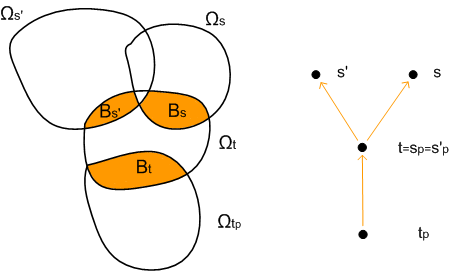
\includegraphics[
            scale=0.30]{Dibujo2.png}}
\end{frame}            

%%%%%%%%%%%%%%%%%%%%%%%%%%%%%%%%%%%%%%%%%%%%%%%%%%%%%%%%%%%%%%%%%%%%%%%%%%%%%%%%%%%%%%%%%%%%%%%%%%%%%%%%%%%%%%%%%%%%%%%%%%%%%%%%%%%%%%%%
%%   Transparencia 9

\begin{frame}\frametitle{$\P_0$-decomposition and tree coverings}

Example 2: $\varphi$ is a H\"older-$\alpha$ function (L'14), $|\varphi(x)=\varphi(y)|\leq C|x-y|^\alpha$. 

\bigskip

\centerline{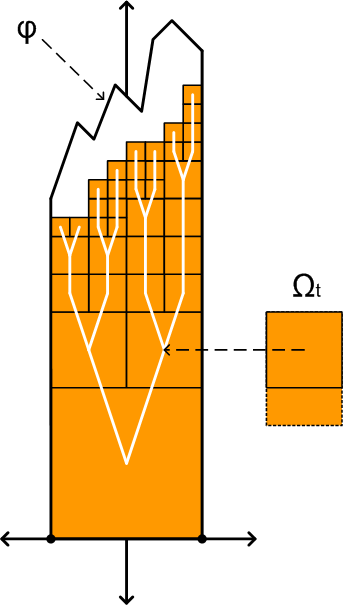
\includegraphics[
            scale=0.25]{Dibujo3.png}}



\end{frame}



%%%%%%%%%%%%%%%%%%%%%%%%%%%%%%%%%%%%%%%%%%%%%%%%%%%%%%%%%%%%%%%%%%%%%%%%%%%%%%%%%%%%%%%%%%%%%%%%%%%%%%%%%%%%%%%%%%%%%%%%%%%%%%%%%%%%%%%%
%%   Transparencia 10

\begin{frame}\frametitle{$\P_0$-decomposition and tree coverings}

Given a tree covering $\{\O_t\}_{t\in\Gamma}$ of $\O$ we define a {\c Hardy type operator} in the following way:
\begin{eqnarray*}
Tg(x):=\sum_{a\neq t\in\Gamma}\dfrac{\chi_{t}(x)}{|W_t|}\int_{W_t}|g|,
\end{eqnarray*} 
where $\displaystyle{W_t=\bigcup_{s\succeq t} \O_s}$ ({\c the shadow of $\O_t$}) and $\chi_t$ is the characteristic function of $B_t$ for all $t\neq a$. 


\end{frame}






%%%%%%%%%%%%%%%%%%%%%%%%%%%%%%%%%%%%%%%%%%%%%%%%%%%%%%%%%%%%%%%%%%%%%%%%%%%%%%%%%%%%%%%%%%%%%%%%%%%%%%%%%%%%%%%%%%%%%%%%%%%%%%%%%%%%%%%%
%%   Transparencia 11

\begin{frame}\frametitle{$\P_0$-decomposition and tree coverings}




\begin{theorem}[L'15] Let $\O\subset\R^n$ be a bounded domain with tree covering $\{\Omega_t\}_{t\in\Gamma}$. Given $g\in L^1(\Omega)$, with $\int_\O g=0$, there exists a  $\P_0$-decomposition $\{g_t\}_{t\in\Gamma}$ of $g$ such that 
\[|g_t(x)| \leq |g(x)|+\frac{|W_t|}{|B_t|}Tg(x).\]
\end{theorem}

Now, if $\frac{|W_t|}{|B_t|}\leq M$ for all $t\neq a$, then 
\begin{eqnarray*}
\sum_{t\in \Gamma} \|g_t\|^q_{L^q(\O_t,\o^{-1})}&=&\sum_{t\in \Gamma} \int_{\O_t}|g_t|^q \o^{-q}\\
&\leq& 2^{q-1}N\left(\|g\|^q_{L^q(\O,\o^{-1})}+M^q\|Tg\|^q_{L^q(\O,\o^{-1})}\right)
\end{eqnarray*}


\end{frame}

%%%%%%%%%%%%%%%%%%%%%%%%%%%%%%%%%%%%%%%%%%%%%%%%%%%%%%%%%%%%%%%%%%%%%%%%%%%%%%%%%%%%%%%%%%%%%%%%%%%%%%%%%%%%%%%%%%%%%%%%%%%%%%%%%%%%%%%%
%%   Transparencia 12

\begin{frame}\frametitle{$\P_0$-decomposition and tree coverings}
\begin{lemma}['15]
$T:L^q(\O)\to L^q(\O)$ is continuous for $1<q\leq \infty$.
\end{lemma}
{\c {Proof:}} 
$T$ is an average of $f$ or zero, thus $\|T\|_{L^\infty\to L^\infty} \leq 1$. 
 \bigskip

$T$ is weak $(1,1)$ continuous with norm lesser than or equal to $N$: 

Given $\lambda>0$, we define the subset of minimal vertices $\Gamma_0\subseteq \Gamma$ as 
\begin{eqnarray*}
\Gamma_0:=\left\{t\in \Gamma\,:\,\frac{1}{|W_t|}\int_{W_t}|f|>\lambda\text{ and }\frac{1}{|W_s|}\int_{W_s}|f|\leq\lambda\text{ for all }s\prec t \right\}.
\end{eqnarray*}

\begin{eqnarray*}
{\rm Thus,}\ \ |\{x\in\O\,:\,Tf(x)>\lambda\}|&\leq& \sum_{t\in \Gamma_0}|W_{t}|\\
&<& \frac{1}{\lambda} \sum_{t\in\Gamma_0}\int_{W_{t}}|f|\leq \dfrac{N}{\lambda} \|f\|_{L^1(\O)}.
\end{eqnarray*}



By Marcinkiewicz interpolation, $\|T\|_{L^q\to L^q} \leq 2\left(\dfrac{qN}{q-1}\right)^{1/q}$.

\vspace{.8cm}
\end{frame}

%%%%%%%%%%%%%%%%%%%%%%%%%%%%%%%%%%%%%%%%%%%%%%%%%%%%%%%%%%%%%%%%%%%%%%%%%%%%%%%%%%%%%%%%%%%%%%%%%%%%%%%%%%%%%%%%%%%%%%%%%%%%%%%%%%%%%%%%
%%   Transparencia 13

\begin{frame}\frametitle{Finding an appropriate covering for John domains}

$\O$ is called a {\c John domain} with parameter $\beta>1$ if there exists a point $x_0\in\O$ such that every $y\in\O$ has a rectifiable curve parameterized by arc length $\gamma:[0,l]\to\Omega$ such that $\gamma(0)=y$, $\gamma(l)=x_0$ and 
\begin{eqnarray*}
\text{dist}(\gamma(t),\partial\O)\geq \frac{1}{\beta}t
\end{eqnarray*}
for all $t\in[0,l]$. Introduced by F. John '61. Named after him by Martio and Sarvas '79.

\bigskip

{\c Examples}: Convex, star-shaped domains with respect to a ball, Lipschitz, Kock snowflake.



\end{frame}


%%%%%%%%%%%%%%%%%%%%%%%%%%%%%%%%%%%%%%%%%%%%%%%%%%%%%%%%%%%%%%%%%%%%%%%%%%%%%%%%%%%%%%%%%%%%%%%%%%%%%%%%%%%%%%%%%%%%%%%%%%%%%%%%%%%%%%%%
%%   Transparencia 14

\begin{frame}\frametitle{Finding an appropriate covering for John domains}

A {\c Whitney decomposition} of $\O$ is a collection $\{Q_t\}_{t\in\Gamma}$ of closed dyadic cubes whose interiors are pairwise disjoint, which verifies
\begin{enumerate}
\item $\O=\bigcup_{t\in\Gamma}Q_t$,
\item $\text{diam}(Q_t) \leq \rho(Q_t,\partial\Omega) \leq 4\text{diam}(Q_t)$,
\item $\frac{1}{4}\text{diam}(Q_s)\leq \text{diam}(Q_t)\leq 4\text{diam}(Q_s)$, if $Q_s\cap Q_t\neq \emptyset$.
\end{enumerate}

\bigskip

A domain $\O$ satisfies the {\c Boman chain condition} if for any cube $Q_t$ in a Whitney decomp. there is a chain $Q_{t,0},\, Q_{t,1},\, \cdots,\, Q_{t,\kappa}$ s.t. $Q_{t,0}=Q_t$,  $Q_{t,\kappa}=Q_a$ (a distinguished cube) and 
\[Q_{t,i}\subset \lambda Q_{t,j},\]
for all $1\leq i\leq j\leq \kappa$. The length of the chain depends on $Q_t$ (Boman '82). 

\end{frame}


%%%%%%%%%%%%%%%%%%%%%%%%%%%%%%%%%%%%%%%%%%%%%%%%%%%%%%%%%%%%%%%%%%%%%%%%%%%%%%%%%%%%%%%%%%%%%%%%%%%%%%%%%%%%%%%%%%%%%%%%%%%%%%%%%%%%%%%%
%%   Transparencia 15

\begin{frame}\frametitle{Finding an appropriate covering for John domains}

Buckley, Koskela and Lu '96: Boman chain condition characterizes John domains.

\bigskip

{\c Boman tree condition:} Given a bounded John domain $\O\subset\R^n$, there exists a Whitney decomposition $\{Q_t\}_{t\in\Gamma}$ where $\Gamma$ has a tree structure that satisfies 
\[Q_s\subseteq K Q_t\]
for any $s,t\in\Gamma$, with $s\succeq t$. We use some ideas from Vasil'eva '13.


\centerline{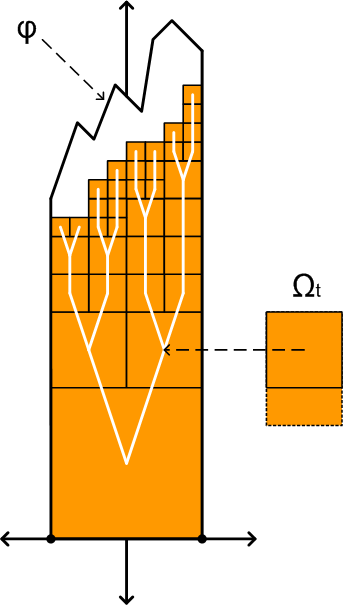
\includegraphics[
            scale=0.15]{Dibujo3.png}}


\end{frame}


%%%%%%%%%%%%%%%%%%%%%%%%%%%%%%%%%%%%%%%%%%%%%%%%%%%%%%%%%%%%%%%%%%%%%%%%%%%%%%%%%%%%%%%%%%%%%%%%%%%%%%%%%%%%%%%%%%%%%%%%%%%%%%%%%%%%%%%%
%%   Transparencia 16

\begin{frame}\frametitle{Finding an appropriate covering for John domains}

Then, there exists a tree covering $\{\O_t\}_{t\in\Gamma}$ of $\O$ such that 
{\c \[|W_t|=|\bigcup_{s\succeq t} \O_s|\leq K^n |\O_t|\leq K^n c_n|B_t|.\]}

Moreover,  using that $\beta\geq 0$, we have $T:L^q(\O,\rho^{-\beta})\to L^q(\O,\rho^{-\beta})$ is continuous with norm {\c $\|T\|\leq C_{n,q,\beta}K^\beta$}.


\bigskip

Thus,  for any  $g\in L^q(\O,\rho^{-\beta})$, with $\int_\O g=0$, there exists a  $\P_0$-decomposition $\{g_t\}_{t\in\Gamma}$ of $g$ such that 
\[|g_t(x)| \leq |g(x)|+\frac{|W_t|}{|B_t|}Tg(x)\leq |g(x)|+c_nK^nTg(x)\]

Which implies 

{\c \[\sum_{t\in \Gamma} \|g_t\|^q_{L^q(\O_t,\rho^{-\beta})}\leq C_{n,q,\beta} K^{q(n+\beta)}\|g\|^q_{L^q(\O,\rho^{-\beta})}\]}

\end{frame}


%%%%%%%%%%%%%%%%%%%%%%%%%%%%%%%%%%%%%%%%%%%%%%%%%%%%%%%%%%%%%%%%%%%%%%%%%%%%%%%%%%%%%%%%%%%%%%%%%%%%%%%%%%%%%%%%%%%%%%%%%%%%%%%%%%%%%%%%
%%   Transparencia 17

\begin{frame}\frametitle{Main Theorem on John domains}

\begin{theorem}\label{Korn in John} Let $\Omega\subset\R^n$ be a bounded John domain with $n\geq 2$, $1<p<\infty$ and $\beta\in\R_{\geq 0}$. Then, there exists a constant $C$ depending only on $n$, $p$ and $\beta$such that  
\begin{eqnarray*}
\left(\int_\Omega |D\uu|^p\rho^{p\beta}\, \d x\right)^{1/p} \leq C\,K^{n+\beta} \left(\int_\Omega |\varepsilon(\uu)|^p\rho^{p\beta}\, \d x\right)^{1/p}
\end{eqnarray*}
for all vector field $\uu\in W^{1,p}(\Omega,\rho^\beta)^n$ that satisfies that $\int_{\O}\eta_{ij}(\uu)\,\rho^{\beta p}=0$, for $1\leq i<j\leq n$. The function $\rho(x)$ is the distance to the boundary of $\Omega$. The constant $K$ appears in the Boman tree condition.
\end{theorem}

\end{frame}

%%%%%%%%%%%%%%%%%%%%%%%%%%%%%%%%%%%%%%%%%%%%%%%%%%%%%%%%%%%%%%%%%%%%%%%%%%%%%%%%%%%%%%%%%%%%%%%%%%%%%%%%%%%%%%%%%%%%%%%%%%%%%%%%%%%%%%%%
%%   Transparencia 18


\begin{frame}\frametitle{$\P_0$-decomposition + Cont. + Local weighted solutions $\Rightarrow$ \\ Weighted solutions of \di\uu=g}

        
  $W^{1,q}(\O):=\left\{v\in L^q(\O)\,:\,\frac{\partial v}{\partial x_i}\in L^q(\O)\text{ for all }i\right\}.$
  
  \bigskip
  
  $W_0^{1,q}(\O):= \overline{C_0^\infty(\O)}\subset W^{1,q}(\O)$.

   \bigskip 
        
        
Given $g\in L^q_0(\Omega)=\left\{g\in L^p(\Omega)\,:\,\int_\Omega g=0\right\}$ there exists $\uu\in W_0^{1,q}(\Omega)^n$ such that 

\[
\di \uu=\,g\]

\[\|D\uu\|_{L^q(\O)}\,\leq\,C\,\|g\|_{L^q(\O)},\]

where $C$ depends only on $\O$ and $q$.
\bigskip 

Note: The existence of a solution of $\di\uu=g$ is basic on the variational analysis of the Stokes equations.


\end{frame}        
        
        
%%%%%%%%%%%%%%%%%%%%%%%%%%%%%%%%%%%%%%%%%%%%%%%%%%%%%%%%%%%%%%%%%%%%%%%%%%%%%%%%%%%%%%%%%%%%%%%%%%%%%%%%%%%%%%%%%%%%%%%%%%%%%%%%%%%%%%%%
%%   Transparencia 19


\begin{frame}\frametitle{$\P_0$-decomposition + Cont. + Local weighted solutions $\Rightarrow$ \\ Weighted solutions of \di\uu=g}

\begin{theorem}
Let $\O\subset\R^n$ be a bounded John domain with $n\geq 2$, $1<q<\infty$ and $\beta\geq 0$. Given $g\in L^q(\O,\rho^{-\beta})$, with $\int_\O g=0$, there exists a solution $\uu\in W^{1,q}_0(\O,\rho^{-\beta})^n$ of $\di\uu=g$ that satisfies
\begin{eqnarray*}
\|D\uu\|_{L^q(\O,\rho^{-\beta})}\leq C_{n,q,\beta} K^{n+\beta} \|g\|_{L^q(\O,\rho^{-\beta})},
\end{eqnarray*}
where $\rho(x)$ is the distance to $\partial\Omega$  and $K$ appears in the Boman tree condition.
\end{theorem}


\end{frame}

  


        
  

%%%%%%%%%%%%%%%%%%%%%%%%%%%%%%%%%%%%%%%%%%%%%%%%%%%%%%%%%%%%%%%%%%%%%%%%%%%%%%%%%%%%%%%%%%%%%%%%%%%%%%%%%%%%%%%%%%%%%%%%%%%%%%%%%%%%%%%%
%%   Transparencia 20


\begin{frame}\frametitle{$\P_0$-decomposition + Cont. + Local weighted solutions $\Rightarrow$ \\ Weighted solutions of \di\uu=g}

{\c Proof:} Given $g\in L^q(\Omega,\rho^{-\beta})\subset L^1(\O)$, with $\int g=0$, we take a $\P_0$-decomposition of $g$ 
(i.e. $g=\sum_t g_t$, $\text{supp}(g_t)\subset \O_t$ and $\int_{\O_t}g_t=0$) and 
\[\sum_{t\in\Gamma}\|g_t\|^q_{L^q(\O_t,\rho^{-\beta})} \leq C_0^q \|g\|^q_{L^q(\O,\rho^{-\beta})}.\]

\bigskip

Next, we take a solution $\uu_t\in W_0^{1,q}(\O_t,\rho^{-\beta})^n$ of $\di\uu_t=g_t$ in $\O_t$ with 
\[\|D\uu_t\|^q_{L^q(\O_t,\rho^{-\beta})} \leq C^q_1 \|g_t\|^q_{L^q(\O_t,\rho^{-\beta})},\]

where $C_1$ is independent of $t$. 

Then, $\uu_t\in W_0^{1,q}(\O,\rho^{-\beta})^n$ by extending by zero. Thus, $\uu=\sum_{t\in\Gamma} \uu_t$ is a solution of $\di\uu=g$ with 


\[\|D\uu\|^q_{L^q(\O,\rho^{-\beta})}\leq C\sum_{t\in\Gamma}\|D\uu_t\|^q_{L^q(\O_t,\rho^{-\beta})} \leq C\sum_{t\in\Gamma}\|g_t\|^q_{L^q(\O_t,\rho^{-\beta})} \leq C \|g\|^q_{L^q(\O,\rho^{-\beta})}\]

\end{frame}

  
%%%%%%%%%%%%%%%%%%%%%%%%%%%%%%%%%%%%%%%%%%%%%%%%%%%%%%%%%%%%%%%%%%%%%%%%%%%%%%%%%%%%%%%%%%%%%%%%%%%%%%%%%%%%%%%%%%%%%%%%%%%%%%%%%%%%%%%%
%%   Transparencia 21

\begin{frame}\frametitle{Question: Upper bounds of the constants on star-shaped domains}

A domain ${\c\O\subset \R^n}$ with diameter {\c $R$} is a star-shaped domain with respect to a ball {\c $B:=B(x_0,\rho)$} if the segment that connects any two arbitrary points $x\in B$ and $y\in \O$ is included in $\O$.

\bs

The estimate of the constant $C_\O$ in the problem $\di\uu=g$, where $\uu\in W^{1,2}_0(\O)^n$, with \[\|D\uu\|_{L^2(\O)}\,\leq\,C_\O\,\|g\|_{L^2(\O)}.\]

\bs

Bogovski '79: Solvability on star-shaped domains. 

\bs 

{\c Can we estimate the constant in terms of the ratio $\dfrac{R}{\rho}$?}

\end{frame}



%%%%%%%%%%%%%%%%%%%%%%%%%%%%%%%%%%%%%%%%%%%%%%%%%%%%%%%%%%%%%%%%%%%%%%%%%%%%%%%%%%%%%%%%%%%%%%%%%%%%%%%%%%%%%%%%%%%%%%%%%%%%%%%%%%%%%%%%
%%   Transparencia 22

\begin{frame}\frametitle{Question: Upper bounds of the constants on star-shaped domains}

Galdi's book '94: {\c$C_\O\leq C_n\,\left(\dfrac{R}{\rho}\right)^{n+1}$}.

\bs

Dur\'an '12: {\c $C_\O\leq C_n\, \dfrac{R}{\rho} \left(\dfrac{|\O|}{|B|}\right)^{\frac{n-2}{2(n-1)}}\left(\log\frac{|\Omega|}{|B|}\right)^{\frac{n}{2(n-1)}}$}.

\bs

In particular, if $n=2$: $C_\O\leq C_n\dfrac{R}{\rho}\log\frac{|\Omega|}{|B|}$.

\bs

Costabel-Dauge '15: For $n=2$, {\c $C_\O=C_n \dfrac{R}{\rho}$}, which is optimal. 

\end{frame}
%%%%%%%%%%%%%%%%%%%%%%%%%%%%%%%%%%%%%%%%%%%%%%%%%%%%%%%%%%%%%%%%%%%%%%%%%%%%%%%%%%%%%%%%%%%%%%%%%%%%%%%%%%%%%%%%%%%%%%%%%%%%%%%%%%%%%%%%
%%   Transparencia 23

\begin{frame}\frametitle{Question: Upper bounds of the constants on star-shaped domains}

{\c Question:}
Given a star-shaped domain $\O\subset\R^n$ as in the previous definition, is there a Whitney decomposition $\O=\bigcup_{t\in\Gamma} \O_t$, where $\Gamma$ is a rooted tree, and a real number $m\geq 1$ such that 
\[\dfrac{\left|\bigcup_{s\succeq t}\O_s\right|}{\left|\O_t\right|}\leq C_n \left(\frac{R}{\rho}\right)^m\]
for all $t\in\Gamma$?

\bigskip

If we have a positive answer to this question, then 
\[C_\O\leq C_n \left(\frac{R}{\rho}\right)^m.\]

\bigskip

What is the infimum the those m's?

\end{frame}


%%%%%%%%%%%%%%%%%%%%%%%%%%%%%%%%%%%%%%%%%%%%%%%%%%%%%%%%%%%%%%%%%%%%%%%%%%%%%%%%%%%%%%%%%%%%%%%%%%%%%%%%%%%%%%%%%%%%%%%%%%%%%%%%%%%%%%%%
%%   Transparencia 24


\begin{frame}\frametitle{Current work: Generalized Korn inequality}

Given $\O\subset\R^n$ with $n\geq 3$,  generalized Korn inequality states:
\[{\c\inf_{l(\ww)=0}\|D\vv-D\ww\|_{L^p(\O)}\leq C \|l(\vv)\|_{L^p(\O)}}\] 
for all $\vv\in W^{1,p}(\O)^n$, where the operator l is the trace free part of $\varepsilon$. Indeed, 
\[l(\uu):=\varepsilon(\uu)-\frac{\di\uu}{n} I_n\]

$l(\ww)=0$ if and only if 
\begin{eqnarray*}
\ww(x)=a+Ax+\lambda x+\left\{\langle b,x\rangle x-\frac{1}{2}|x|^2b\right\},
\end{eqnarray*}

where $a,b\in\R^n$, $\lambda\in\R$ and $A\in\R^{n\times n}$ is skew-symmetric.

\bigskip

Note: We have to consider $V$-orthogonal decomposition for another vector space $V$ different from $\P_0$.

\end{frame}






%%%%%%%%%%%%%%%%%%%%%%%%%%%%%%%%%%%%%%%%%%%%%%%%%%%%%%%%%%%%%%%%%%%%%%%%%%%%%%%%%%%%%%%%%%%%%%%%%%%%%%%%%%%%%%%%%%%%%%%%%%%%%%%%%%%%%%%%%
%%   Transparencia  25

\begin{frame}\frametitle{}


\begin{center}
\textbf{\Large Thanks for your attention!}
\end{center}
\end{frame}


\end{document}
